% !TEX root = Document.tex
%!TeX spellcheck = fr
\Chapter{REVUE DE LITTÉRATURE}\label{sec:RevLitt}
%
%\color{red}
%Bien que les deux types d'inspections traités dans ce mémoire sont exécutés sur des véhicules entièrement différents, les concepts utilisées lors de ces opérations se recoupent énormément. Dans ce chapitre nous présentons d'abord dans la section \ref{subsec:positionnement} diverses méthodes de positionnement couramment utilisées par les robots mobiles pour naviguer dans leur environnement. Dans le même ordre d'idée nous présentons ensuite dans la section \ref{subsec:reconstruction} diverses façons pour un robot de résoudre le problème de \textit{Simultaneous Localization and Mapping} (SLAM) pour calculer la position relative du robot dans son environnement. La section \ref{subsec:generation} présente l'état de l'art en termes de génération de trajectoires pour la couverture de surfaces et de volumes.
%%Puis la section \ref{subsec:navigation} présente quelques algorithmes couramment utilisés pour la navigation de robots mobiles.
%Finalement dans la section \ref{subsec:eolienne} nous abordons le sujet spécifique de l'inspection d'éoliennes au moyen de robots autonomes.
%\color{black}

Bien que les deux types d'inspections traités dans ce mémoire sont exécutés sur des véhicules entièrement différents, les concepts utilisées lors de ces opérations se recoupent énormément. Dans ce chapitre, nous présentons d'abord dans la section \ref{subsec:generation} le travail antérieur directement en lien avec la génération de trajectoires d'inspection. Par la suite, nous traitons du sujet plus spécifique d'inspection d'éoliennes au moyens de robots aériens autonomes dans la section \ref{subsec:eolienne}. Ensuite nous présentons les théories et les méthodes connexes requises pour l'opération des robots dans des environnements inconnus, en particulieur les méthodes de positionnement dans la section \ref{subsec:positionnement} et les méthodes de localisation et cartographier simultanée dans la section \ref{subsec:reconstruction}. Finalement, nous terminons la revue de littérature par un survol des capteurs couramment utilisés pour la navigation de robots autonomes dans la section \ref{sec:capteurs}.

\section{Génération de trajectoires d'inspection et couverture de surfaces}\label{subsec:generation}

En général, le but des générateurs de trajectoire est d'optimiser une certaine métrique permettant de décider à quel endroit il faut placer le véhicule et son capteur pour faire l'inspection de la structure. Tout d'abord, considérons le cas d'une mission sans information \textit{a priori}. Il s'agit d'une mission d'exploration où la génération de trajectoires doit se faire itérativement en temps réel pour envoyer le robot aux confins de l'espace connu. On tente en fait de répondre à la question:

\begin{quote}
  \emph{Given what you know about the world, where should you move to gain as much new information as possible?} (Sachant ce que nous savons à propos du monde, où devrions nous aller pour gagner le plus d'information possible?) \citep{Yamauchi1997}.
\end{quote}

Pour ce faire, Yamauchi introduit le concept de \textit{frontier-based exploration} qui cherche à guider un robot vers la frontière entre l'espace connu et libre, et l'espace inconnu. Suivant cette idée plusieurs chercheurs proposent des fonctions de coût à minimiser permettant de choisir à quel endroit de la frontière explorer. \citep{Wirth2007} proposent de subdiviser une carte 2D en cellules pour lesquelles une fonction de coût est calculée en prenant en compte non seulement la plus courte distance par rapport au robot mais aussi la distance par rapport à l'obstacle le plus proche. Chaque nouvelle position objectif minimise ainsi la distance pour s'y rendre mais aussi le risque encouru par le robot. Au lieu d'utiliser les frontières comme objectifs \citep{Dornhege2011} proposent une formulation du problème utilisant les frontières en tant que candidates possibles d'ouvertures dans les murs qui permettraient à une caméra de cartographier l'espace vide se trouvant derrière.

\citep{Bircher2016} proposent une méthode d'exploration 3D basée sur l'algorithme \textit{Rapidly exploring Random Trees} (RRT) où un arbre est construit dans l'espace ouvert connu. À chaque sommet, l'angle de vue de la caméra est utilisé pour estimer le gain exploratoire de la position. Une fois l'arbre construit, le véhicule exécute la première étape de la branche possédant le plus grand gain total. L'arbre complet est ensuite recalculé en utilisant la branche choisie comme point de départ. En d'autres mots, leur méthode tente de maximiser le gain exploratoire en prenant aussi en compte les gains futurs d'une trajectoire. Outre les gains exploratoires, certains auteurs tentent aussi de prendre en compte l'effet des trajectoires sur leurs systèmes de navigation. Par exemple \citep{Papachristos2017} améliorent la méthode de Bircher en sélectionnant un trajectoire qui permet aussi de minimiser l'incertitude sur leur système de cartographie et d'odométrie visuelle. \citep{Wirth2007} notent d'ailleurs que la proximité d'un obstacle est un danger (de collision) mais l'éloignement des obstacles en est aussi puisque la portée limitée des capteurs pourrait rendre un système de SLAM temporairement aveugle.

Alors que les méthodes précédentes se préoccupent de maximiser le gain d'information, elles ne prennent pas en compte les contraintes de temps liées à l'autonomie des robots, un problème qui affecte grandement les véhicules aériens multi-rotors. En combinant une fonction d'entropie calculée dans un voisinage local avec le coût en distance d'une trajectoire, \citep{Wang2017} proposent une méthode d'exploration se basant sur les \textit{Information Potential Fields} (les champs de potentiels d'information). Similaire à la méthode des champs de potentiels pour l'évitement d'obstacles, le robot finit par être attiré dans les régions les plus proches à haut gain d'information. Toutefois, minimiser la longueur de la trajectoire n'assure pas nécessairement une minimisation du temps d'exploration si nous prenons aussi en compte l'accélération ou le jerk requis pour exécuter celle-ci. Pour résoudre ce problème \citep{Cieslewski2017} proposent une extension de la méthode de \citep{Yamauchi1997} où la prochaine frontière est choisie est sélectionnée dans le champ de vision du véhicule de telle sorte qu'il minimise le changement de vitesse requis pour le robot. Ainsi, la trajectoire exécutée peut être plus longue que les méthodes conventionnelles mais elle permet de maintenir une vitesse de navigation plus élevée.

Il est toutefois important de noter que ces méthodes d'inspection basées sur une variante de l'exploration de frontières ne se préocuppent pas d'assurer la couverture totale d'une structure spécifique mais elles cherchent plutôt à explorer un certain espace ou un volume. Les méthodes d'inspection que nous proposons visent spécifiquement l'inspection de la surface atteignable d'une structure fermée.

Dans un autre ordre d'idée, une trajectoire complète et globalement optimale peut être générée au préalable si de l'information \textit{a priori} est disponible. Pour une mission où la géométrie de la structure à inspecter est connue, \citep{Bircher2015} proposent de résoudre le problème en deux temps. En subdivisant le modèle en un maillage de triangles, on obtient pour chaque face un ensemble de points de vues admissibles. À chaque itération, des points de vue sont choisis séquentiellement en résolvant un problème d'optimisation QP (\emph{Quadratic Programming}) où la fonction de coût minimise la distance par rapport aux points de vue voisins et où les contraintes assurent que la surface soit visible par le véhicule. Une fois l'ensemble choisi, une recherche heuristique est effectuée pour résoudre un problème de type commis voyageur à travers l'ensemble. Bircher réexécute les deux étapes jusqu'à ce qu'une trajectoire satisfaisante soit trouvée. \citep{sheng2008crawler} utilisent un modèle CAD d'un aéronef pour planifier une trajectoire permettant d'inspecter tous les rivets à la surface du véhicule. \citep{Yoder2016} débutent plutôt avec une boite de délimitation 3D autour de la structure pour ensuite faire une exploration par frontière de surface.

Comparativement à l'inspection par exploration (en temps réel) la génération de trajectoires hors-ligne permet de créer des plans optimaux en termes de temps et de distance à parcourir. Par contre, cette trajectoire peut avoir un risque de collision s'il s'avère que le modèle utilisé diffère de la structure réelle, par exemple dans la cas d'un édifice partiellement endommagé par un désastre naturel ou une variation dans l'angle des pales d'une éolienne. \citep{Hepp2017} présentent un système faisant une première passe à haute altitude pour construire une carte rudimentaire dans laquelle la seconde inspection de près est planifiée suivant une maximisation du gain d'information.

Tel que mentionné brièvement précédemment, le travail que nous effectuons est aussi relié au problème de la planification de trajectoire pour la couverture de surface qui, par le passé, a surtout été étudié dans le domaine 2D et supposent normalement un système de localisation précis \citep{Hert1996, acar2002morse, Acar2002, lim2014crack}. Nous soulignons que notre contribution n'est pas de l'avancement théorique de ces méthodes de couverture. Nous proposons plutôt des solutions pratiques permettant de mettre en \oe uvre ces systèmes dans des situations réelles en présence de bruit de localisation et de capteurs.

\section{Méthodes automatiques d'inspection d'éoliennes}\label{subsec:eolienne}

L'inspection d'éoliennes par UAV autonome étant une application relativement nouvelle, peu de travaux ont été publiés sur ce sujet particulier et à ce jour, la majorité du travail accompli demeure théorique, en simulation seulement ou en environnement à petite échelle. Avant tout, \citep{Zhang2014} démontrent la faisabilité de repérer automatiquement des fissures sur la surface d'une éolienne au moyen de détecteurs de bordures bien connus Canny et Sobel. Un travail préliminaire a été réalisé sur les éléments de base requis pour faire une inspection autonome. Notamment au niveau de l'utilisation du principe du flux optique pour l'estimation de la vitesse relative entre un véhicule aérien et une éolienne \citep{Hoglund2014} ainsi que l'utilisation de la transformée de Hough linéaire et de traitements géométriques pour la reconnaissance automatique d'éoliennes \citep{Stokkeland2015}. Stokkeland explique qu'une inspection entièrement visuelle est difficile à réaliser dû à la grande quantité de bruit et de sources d'erreurs présentes sur le terrain. Par exemple, la segmentation entre la surface blanche de l'éolienne et les nuages en arrière plan est extrêmement sensible au réglage des paramètres du filtre de couleur. C'est pourquoi \citep{Heggem2017} fait usage de vision active au moyen d'un projecteur laser et de caméras stéréo pour détecter la distance et la forme de la pale. Avec projection de seulement 11x11 points, Heggem parvient ensuite à calculer dans quelle direction son UAV doit se diriger pour poursuivre son inspection.

Du côté commercial, peu de compagnies se sont aventurées dans le domaine \footnote{Nous notons la présence de SkySpecs aux États-Unis, Pro-Drones en Italie et Perceptual Robotics en Angleterre.} mais tous semblent faire usage de radars lasers et de caméras sous une forme ou une autre.

\section{Méthodes de positionnement}\label{subsec:positionnement}

Selon \citep{Borenstein1997} les systèmes de positionnement se regroupent dans l'une de deux catégories suivantes:
\begin{enumerate}
  \item Les systèmes absolus fonctionnant grâce à de l'information externe tel que les GNSS reposant sur les données de satellites.
  \item Les systèmes à l'estime fonctionnant par l'intégration d'une mesure à travers le temps tel que l'odométrie provenant des roues d'un robot ou la double intégrale d'une accélération pour estimer une position.
\end{enumerate}

\subsection{Systèmes de positionnement inertiel et par GNSS}

Les systèmes de navigation complets vont habituellement se doter d'une combinaison des deux types de capteurs pour obtenir une estimation de la pose (position et orientation) du robot dans l'espace. Les systèmes de positionnement absolus tel que le GPS ayant normalement des fréquences de mise à jour lentes, autour de 1 Hz, ils sont souvent jumelés à une centrale inertielle (IMU), c'est-à-dire une combinaison de gyroscopes et d'accéléromètres permettant de mesurer la vitesse angulaire et l'accélération d'un corps rigide \citep{Noureldin2013}. Bien que les capteurs inertiels permettent d'estimer la position à de hautes fréquences, parfois même 1 kHz, en prenant l'intégrale de ceux-ci, une accumulation d'erreur peut rapidement faire diverger l'estimation d'état. Ainsi, un système inertiel à l'estime et un système GPS absolut jouent des rôles complémentaires où le système inertiel calcule la position à haute fréquence puis une correction est faite par GPS à basse fréquence.

On appelle tout système reposant sur des capteurs inertiels un Système de Navigation Inertiel (INS). De nos jours, ceux-ci sont faciles d'accès et peuvent êtres achetés pour quelques milliers de dollars. La fusion de ces différents capteurs peut se faire au travers de différents moyens tels que les filtres à particules \citep{Carvalho1997} ou les graphes de facteurs \citep{Indelman2012} mais l'outil normalement utilisé est le filtre de Kalman \citep{Noureldin2013}.

Le filtre de Kalman (KF) de base est un algorithme récursif permettant de faire une estimation aux moindres carrés d'un vecteur d'état au travers d'une procédure de prédiction de l'évolution du vecteur d'état suivant un modèle du système suivi de la correction de celui-ci par les mesures entrant dans le filtre. Cet algorithme fonctionne pourvu que la transformation entre l'état et les mesures en entrée soit linéaire. Dans le cas d'un système non linéaire, une linéarisation par un développement de Taylor autour de l'estimé optimal courant du vecteur d'état est effectuée, résultant en un filtre de Kalman étendu (EKF) \citep{Chui2017}.

Les GNSS n'étant pas la seule façon de corriger l'erreur cumulative d'un INS, certains auteurs proposent des filtres de Kalman modulaires permettant de fusionner une quantité arbitraire de capteurs hétérogènes tels que des IMU, l'odométrie d'encodeurs de roues, l'odométrie visuelle, receveurs GNSS, etc. \citep{MooreEkf2014} pour estimer la position et l'orientation du robot. Pour le cas spécifique des UAV \citep{Lynen2013} proposent aussi une architecture modulaire pour un filtre de Kalman étendu itéré qui permet de faire une calibration inter-capteurs en ligne pour estimer les délais temporels et les différences d'échelle des mesures, chose importante dans le cas d'odométrie visuelle monoculaire où l'échelle des mesures est arbitraire et peut dériver avec le temps.

\section{\textit{Simultaneous Localization and Mapping}}\label{subsec:reconstruction}

Les GNSS permettent de localiser un robot sur la surface de la terre, mais qu'en est-il des situations dépourvues de réception satellite adéquate tel que les environnements intérieurs ou les \guillemotleft canyons urbains \guillemotright ? De plus, nous sommes souvent plus intéressés à savoir la position du robot par rapport à son environnement plutôt que sa latitude et longitude. Nous cherchons donc à répondre à \guillemotleft Comment localiser un robot dans son environnement sans une carte de celle-ci?\guillemotright; Une question qui est l'essence du problème de localisation et cartographie simultanée (SLAM).

Un système de SLAM cherche donc à créer une représentation de l'environnement pour ensuite s'y localiser. Cette représentation peut prendre plusieurs formes dépendant du capteur utilisé mais elle cherche habituellement à extraire des points de repère de l'environnement pour former une carte dans laquelle le robot sera localisé. Pour une caméra RGB ces points de repère pourraient être des caractéristiques visuelles extraites des images \citep{Mur-Artal2017}. Une particularité des systèmes de SLAM entièrement visuel et monoculaire est que la carte construite sera à une échelle arbitraire et ne peut donc pas être utilisée pour la navigation d'un robot. Ces dernières années beaucoup de travail a été réalisé pour combiner une caméra monoculaire à une centrale inertielle pour résoudre cette ambiguïté d'échelle \citep{muratal2017vimonoslam}. Une autre façon d'éviter le problème est d'utiliser une caméra RGB-D ou une caméra stereo où la forme des objets en plus des caractéristiques visuelles peut-être utilisée pour cartographier \citep{henry2014rgb}. \citep{Zhang2017} montrent que du SLAM peut aussi être réalisé grâce à un lidar 3D en faisant l'extraction de caractéristiques planaires et de contours.

Bref, une multitude d'approches existent pour l'extraction des points de repère mais ces données seules ne sont pas suffisantes pour la localisation du robot. Les données captées doivent ensuite être traitées par un quelconque mécanisme d'estimation d'état. \citep{Grisetti2010} expliquent que les systèmes se séparent habituellement en deux catégories, ceux par filtrage et ceux par optimisation (Grisetti réfère au \textit{lissage}). Les systèmes par filtre cherchent à estimer l'état courant du robot par rapport à la carte et peuvent utiliser par exemple un filtre à particules \citep{Grisetti2007} ou un EKF \citep{Montemerlo03a}. En revanche, les méthodes par optimisation cherchent à estimer la trajectoire complète du robot au moyen de l'ensemble complet des observations qu'il a recueilli. Pour ce faire, il est intuitif de modéliser le problème de SLAM par un graphe de poses où les connexions entre les noeuds représentent des observations de l'environnement. Ces observations imposent donc des contraintes sur le graphe sur lequel nous cherchons à effectuer une minimisation de l'erreur suivant une formulation par moindres carrés. Cette méthode est utilisé par beaucoup des systèmes de SLAM proposés récemment \citep{Labbe2014, Hess2016}.

Une composante importante de tout système de SLAM est sa capacité de fermeture de boucle, c'est-à-dire d'être capable de reconnaître quand le robot retourne à un endroit déjà visité, particulièrement en l'absence de systèmes de positionnement absolus. Ceci peut être fait localement sur un sous-ensemble local des observations courantes ou globalement sur toutes les observations faites jusqu'au présent. Ceci peut être réalisé d'une variété de façons dépendamment des capteurs utilisés par l'algorithme de SLAM. \citep{Hess2016} proposent Google Cartographer une approche hybride fonctionnant par scanner laser, où les nouveaux balayages sont insérés et appariés par rapport à une sous-carte locale alors que la recherche de fermeture de boucle globale est exécutée en arrière plan par un algorithme de séparation et d'évaluation progressive (\textit{branch-and-bound}). En revanche RTAB-MAP \citep{Labbe2014} utilisent une approche par sac-de-mots (\textit{bag-of-words}) appliquée à des descripteurs extraits d'une image couleur. Pour assurer une opération en temps réel les n\oe uds du graphe de pose, contenant aussi les mots visuels extraits à chaque endroit, sont séparés dans différentes mémoires: la mémoire court terme, la mémoire de travail et la mémoire long terme. Seuls les noeuds dans la mémoire de travail sont considérés pour la fermeture de boucle. Dans les deux cas de Google Cartographer et RTAB-Map, il est donc possible que la détection de la fermeture de boucle échoue si la pose estimée courante du robot a trop dérivé au point que les algorithmes ne cherchent plus à apparier l'environnement courant avec les éléments de la carte connue.

Le but de la fermeture de boucle est de réduire les erreurs de localisation en imposant certaines contraintes sur la carte en cours de construction. Cette minimisation d'erreur peut-être réalisée de plusieurs façons, notamment par optimisation de graphe de poses \citep{Carlone2016}, par compensation par faisceaux (\textit{Bundle Adjustment}) \citep{Mei2011} ou tel que proposé dans ORB-SLAM2 une combinaison des deux \citep{Mur-Artal2017}.

\section{Méthodes de représentation de l'environnement}\label{subsec:representations}

Pour faire naviguer un robot mobile dans un environnement inconnu il est impératif d'avoir une représentation de l'environnement dans laquelle la planification de trajectoire et la vérification de collision est possible. L'important est d'utiliser la représentation appropriée correspondante aux mouvements possibles du robot. Pour la navigation en 3D le cadriciel OctoMap de \citep{Hornung2013} est particulièrement populaire de par son code à source ouverte, sa représentation probabiliste de l'environnement connu et inconnu et son efficacité en termes de mémoire. Une OctoMap représente l'espace volumique par une Octree, subdivisant ainsi récursivement l'espace par un arbre d'octants. Chaque niveau de l'arbre représente une résolution différente de l'espace tel que l'on peut voir dans la Figure \ref{fig:octree}.

\begin{figure}[h]
  \centering
  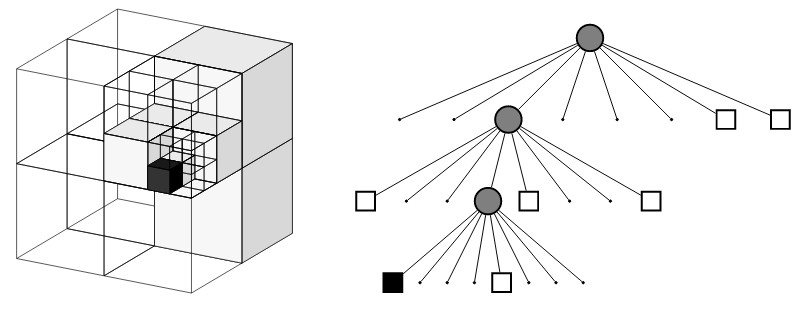
\includegraphics[width=0.5\linewidth]{images/octree.jpg}
  \caption[Représentation graphique d'une Octree]{L'octree est une structure en arbre souvent utilisé pour partitionner un espace tridimensionnel. Figure prise de \citep{Hornung2013}.}
  \label{fig:octree}
\end{figure}

La structure Octree rend l'OctoMap particulièrement efficace en termes de mémoire comparativement à une séparation naïve de l'espace en voxels car l'arbre n'est étendu qu'au besoin. Alors que certaines représentations de l'espace utilisent une forme binaire où tout voxel est soit occupé ou libre, OctoMap utilise une forme probabiliste où chaque voxel est inconnu ou a une probabilité d'être occupé ou libre permettant donc l'OctoMap de représenter l'incertitude et le bruit de mesure sur le capteur utilisé pour construire la carte. Nous avons la probabilité $P(n|z_{1:t})$ qu'une feuille $n$ de l'Octree soit occupée étant donné les mesures de capteurs $z_{1:t}$ est estimé selon
\begin{align}
  P(n|z_{1:t}) = \Bigg[ 1 +
    \frac{1 - P(n|z_{t})}{P(n|z_{t})}
    \frac{1 - P(n|z_{1:t-1})}{P(n|z_{1:t-1})}
    \frac{P(n)}{1 - P(n)}
  \Bigg]^{-1}
  \label{eq:octomap_probability}
\end{align}
avec la probabilité par défaut $P(n) = 0.5$. Les probabilités des voxels peuvent ensuite être dicrétisées pour définitir l'espace vide ($P(n) < 0.12$), l'espace inconnu ($P(n) \in [0.12, 0.97]$) et l'espace occupé ($P(n) > 0.97$) pour appliquer divers algorithmes de génération de trajectoire tel que les RRT ou A*.

Par contre, une OctoMap n'est pas particulièrement bien adapté aux méthodes de planification de trajectoire par optimisation qui ont besoin de savoir la distance aux obstacles en tout point de la carte ainsi que les gradients de distance \citep{ratliff2009chomp, Oleynikova2016}. Ce calcul pouvant être coûteux, \citep{oleynikova2017voxblox} propose d'utiliser une représentation des surface par des fonctions de distance signées tronquées offrant une accélération par la suite dans le calcul des champs de distance euclidiennes signées.

Dans un autre ordre d'idées \citep{Fridovich-Keil2017AtomMap} abandonnent complètement la représentation par grille et proposent d'utiliser des sphères (des \guillemotleft atomes \guillemotright) organisés dans un arbre $k$-d. Ceci permet une représentation plus précise de l'espace libre tangent aux surfaces en plus de faire l'estimation de fonctions de distance signées en temps réel.

%\section{Méthodes de navigation}\label{subsec:navigation}

%\begin{enumerate}
%  \item champs de potentiel
%  \item rrt
%  \item a star
%\end{enumerate}

\section{Traitement d'images}

\subsection{Modèle de caméra}
\label{subsec:modele_camera}
Il arrive souvent dans des applications de traitement d'images de devoir passer du domaine 3D à 2D et vice-versa. Pour ce faire, il est important de passer en revue les modèles de projection et de distorsion d'images couramment utilisés. Tout point 3D $p_w$ à coordonnées connues peut être projeté sur le plan image en un point dont les coordonnées en pixels $\boldsymbol{x_s}$ sont données par l'équation \ref{eq:pinhole_projection}.
\begin{align}
\boldsymbol{x_s} = K[R|t]p_w = P p_w
\label{eq:pinhole_projection}
\end{align}
où $P \in \mathbb{R}^{3\times 4}$ désigne la matrice de caméra, $K \in \mathbb{R}^{3\times3}$ la matrice des paramètres intrinsèques, $R\in \mathbb{R}^{3\times3}$ est une rotation orthogonale et $t$ une translation. Dépendamment des auteurs, $K$ peut être posé différemment; l'équation \ref{eq:intrinsics} présente sa forme générale où $f_x$ et $f_y$ désignent la distance focale en pixels, $(c_x, c_y)$ le centre optique en pixels, $s$ le \textit{skew} prenant en compte l'angle possible entre les axes du capteur et les axes optiques, et finalement $\alpha$ le facteur de forme.
\begin{align}
  K = \begin{bmatrix}
  f_x & s & c_x \\
  0   & \alpha f_y & c_y \\
  0  &  0  & 1
\end{bmatrix}
\label{eq:intrinsics}
\end{align}
En pratique la majorité des applications telle quel la librairie de traitement d'images OpenCV vont simplifier $K$ au moyen de $s = 0$ et $\alpha = 1$ \citep{itseez2015}. Il est aussi utile de passer aux coordonnées homogènes au moyen d'une matrice $\boldsymbol{\tilde{P}} \in \mathbb{R}^{4\times4}$ en ajoutant une ligne à $P$,
\begin{align}
  \boldsymbol{\tilde{P}} = \begin{bmatrix}K & \boldsymbol{0} \\ \boldsymbol{0} & 1\end{bmatrix}
  \begin{bmatrix}R & t \\ \boldsymbol{0} & 1\end{bmatrix} = \boldsymbol{\tilde{K}} \boldsymbol{E}
    \label{eq:homogeneous_projection}
\end{align}
où $\boldsymbol{E}$ est une matrice de transformation 3D. La projection se fait de la même façon que l'équation \ref{eq:pinhole_projection} avec $\boldsymbol{\bar{p}_w} = \begin{bmatrix}p_w^\top & 0 \end{bmatrix}^\top$ et $\boldsymbol{x_s} = \begin{bmatrix}x_s & y_s & 1 & d\end{bmatrix}^\top$
\begin{align}
  \boldsymbol{x_s} \sim \boldsymbol{\tilde{P}} \boldsymbol{\bar{p}_w}
\end{align}
où le symbole $\sim$ indique une égalité à l'échelle et $\boldsymbol{x_s}$ doit être normalisé après la multiplication pour que la troisième composante soit $1$ \citep{Szeliski2011}.

Ces formules sont valides dans le cas de projections entièrement linéaires. En revanche les systèmes optiques vont habituellement introduire une certaine distorsion de l'image, surtout dans le cas de lentilles grand angle.
% Par exemple dans la Figure \ref{fig:distortion} les lentilles de la caméra Zed avec un angle de vue de $110^\circ$ (D) introduisent beaucoup de distorsion courbant ainsi des lignes qui devraient normalement être droites.

%\begin{figure}[htp]
%  \centering
%  \begin{minipage}{0.4\textwidth}
%    \centering
%    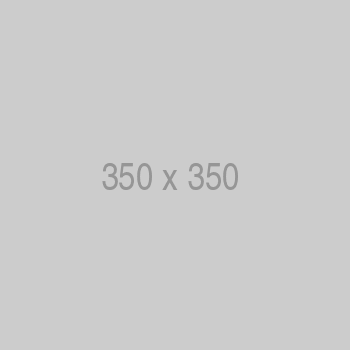
\includegraphics[width=\linewidth]{images/placeholder.png}
%    (A)
%  \end{minipage}
%  \begin{minipage}{0.4\textwidth}
%    \centering
%    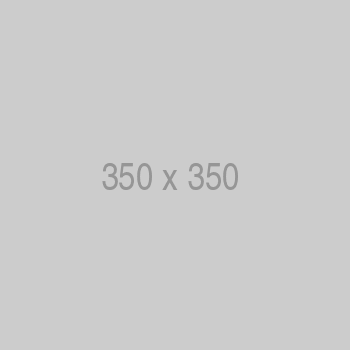
\includegraphics[width=\linewidth]{images/placeholder.png}
%    (B)
%  \end{minipage}
%  \caption{Exemple de distorsion introduite par une lentille à grand angle. (A) l'image originale (B) l'image %rectifiée}
%  \label{fig:distortion}
%\end{figure}

Plusieurs modèles de distorsion ont été proposés à travers le temps mais le plus répandu est le modèle radial-tangentiel, radial puisqu'il dépend de la distance du pixel par rapport au centre optique, et tangentiel pour le déplacement des rayons tangents au cercle autour du centre optique. La distorsion radiale-tangentielle peut-être exprimée par un polynôme permettant de mettre en correspondance les pixels de l'image originale $(x_c, y_c)$ en coordonnées normalisées aux pixels de l'image rectifiée $(u, v)$:
\begin{equation}
  \begin{aligned}
    \hat{x}_c &= x_c\left(\frac{1 + \kappa_1r_c^2 + \kappa_2r_c^4 + \kappa_3r_c^6}{1 + \kappa_4r_c^2 + \kappa_5r_c^4 + \kappa_6r_c^6}\right) + 2p_1 x_c y_c + p_2(r_c^2 + 2 x_c^2) \\
    \hat{y}_c &= y_c\left(\frac{1 + \kappa_1r_c^2 + \kappa_2r_c^4 + \kappa_3r_c^6}{1 + \kappa_4r_c^2 + \kappa_5r_c^4 + \kappa_6r_c^6}\right) + p_1 (r_c^2 + 2 y_c^2) + 2p_2 x_c y_c \\
    r_c^2     &= x_c^2 + y_c^2
    \label{eq:rectification}
  \end{aligned}
\end{equation}
et
\begin{equation}
  \begin{aligned}
    u & = f_x \hat{x}_c + c_x\\
    v &= f_y \hat{y}_c + c_y
    \label{eq:focal_scaling}
  \end{aligned}
\end{equation}
Les paramètres $\kappa_{[1-6]}$ sont les coefficients de distorsion radiaux et $p_{[1,2]}$ les coefficients de distorsion tangentiels. L'équation \ref{eq:focal_scaling} permet de mettre à l'échelle les coordonnées normalisées en coordonnées en pixels. Les paramètres de distorsion et intrinsèques peuvent être estimés conjointement suivant la résolution d'un problème des moindres carrés non-linéaire \citep{Zhang2000}.

Bien que le modèle radial-tangentiel soit le plus populaire, entres autres par sa présence dans la librairie de traitement d'images OpenCV, plusieurs auteurs proposent de nouveaux modèles avec divers avantages. Par exemple le modèle de distorsion équidistant proposé par \citep{Kannala2006} est apte à modéliser la distorsion à la fois de lentilles normales et de lentilles ultra-grand angle et le modèle par fonction rationnelle de \citep{Claus2005} adapté aux lentilles grand-angle et catadioptriques.

\subsection{Vision stéréo}\label{subsec:stereo_vision}

\begin{figure}[h]
  \centering
  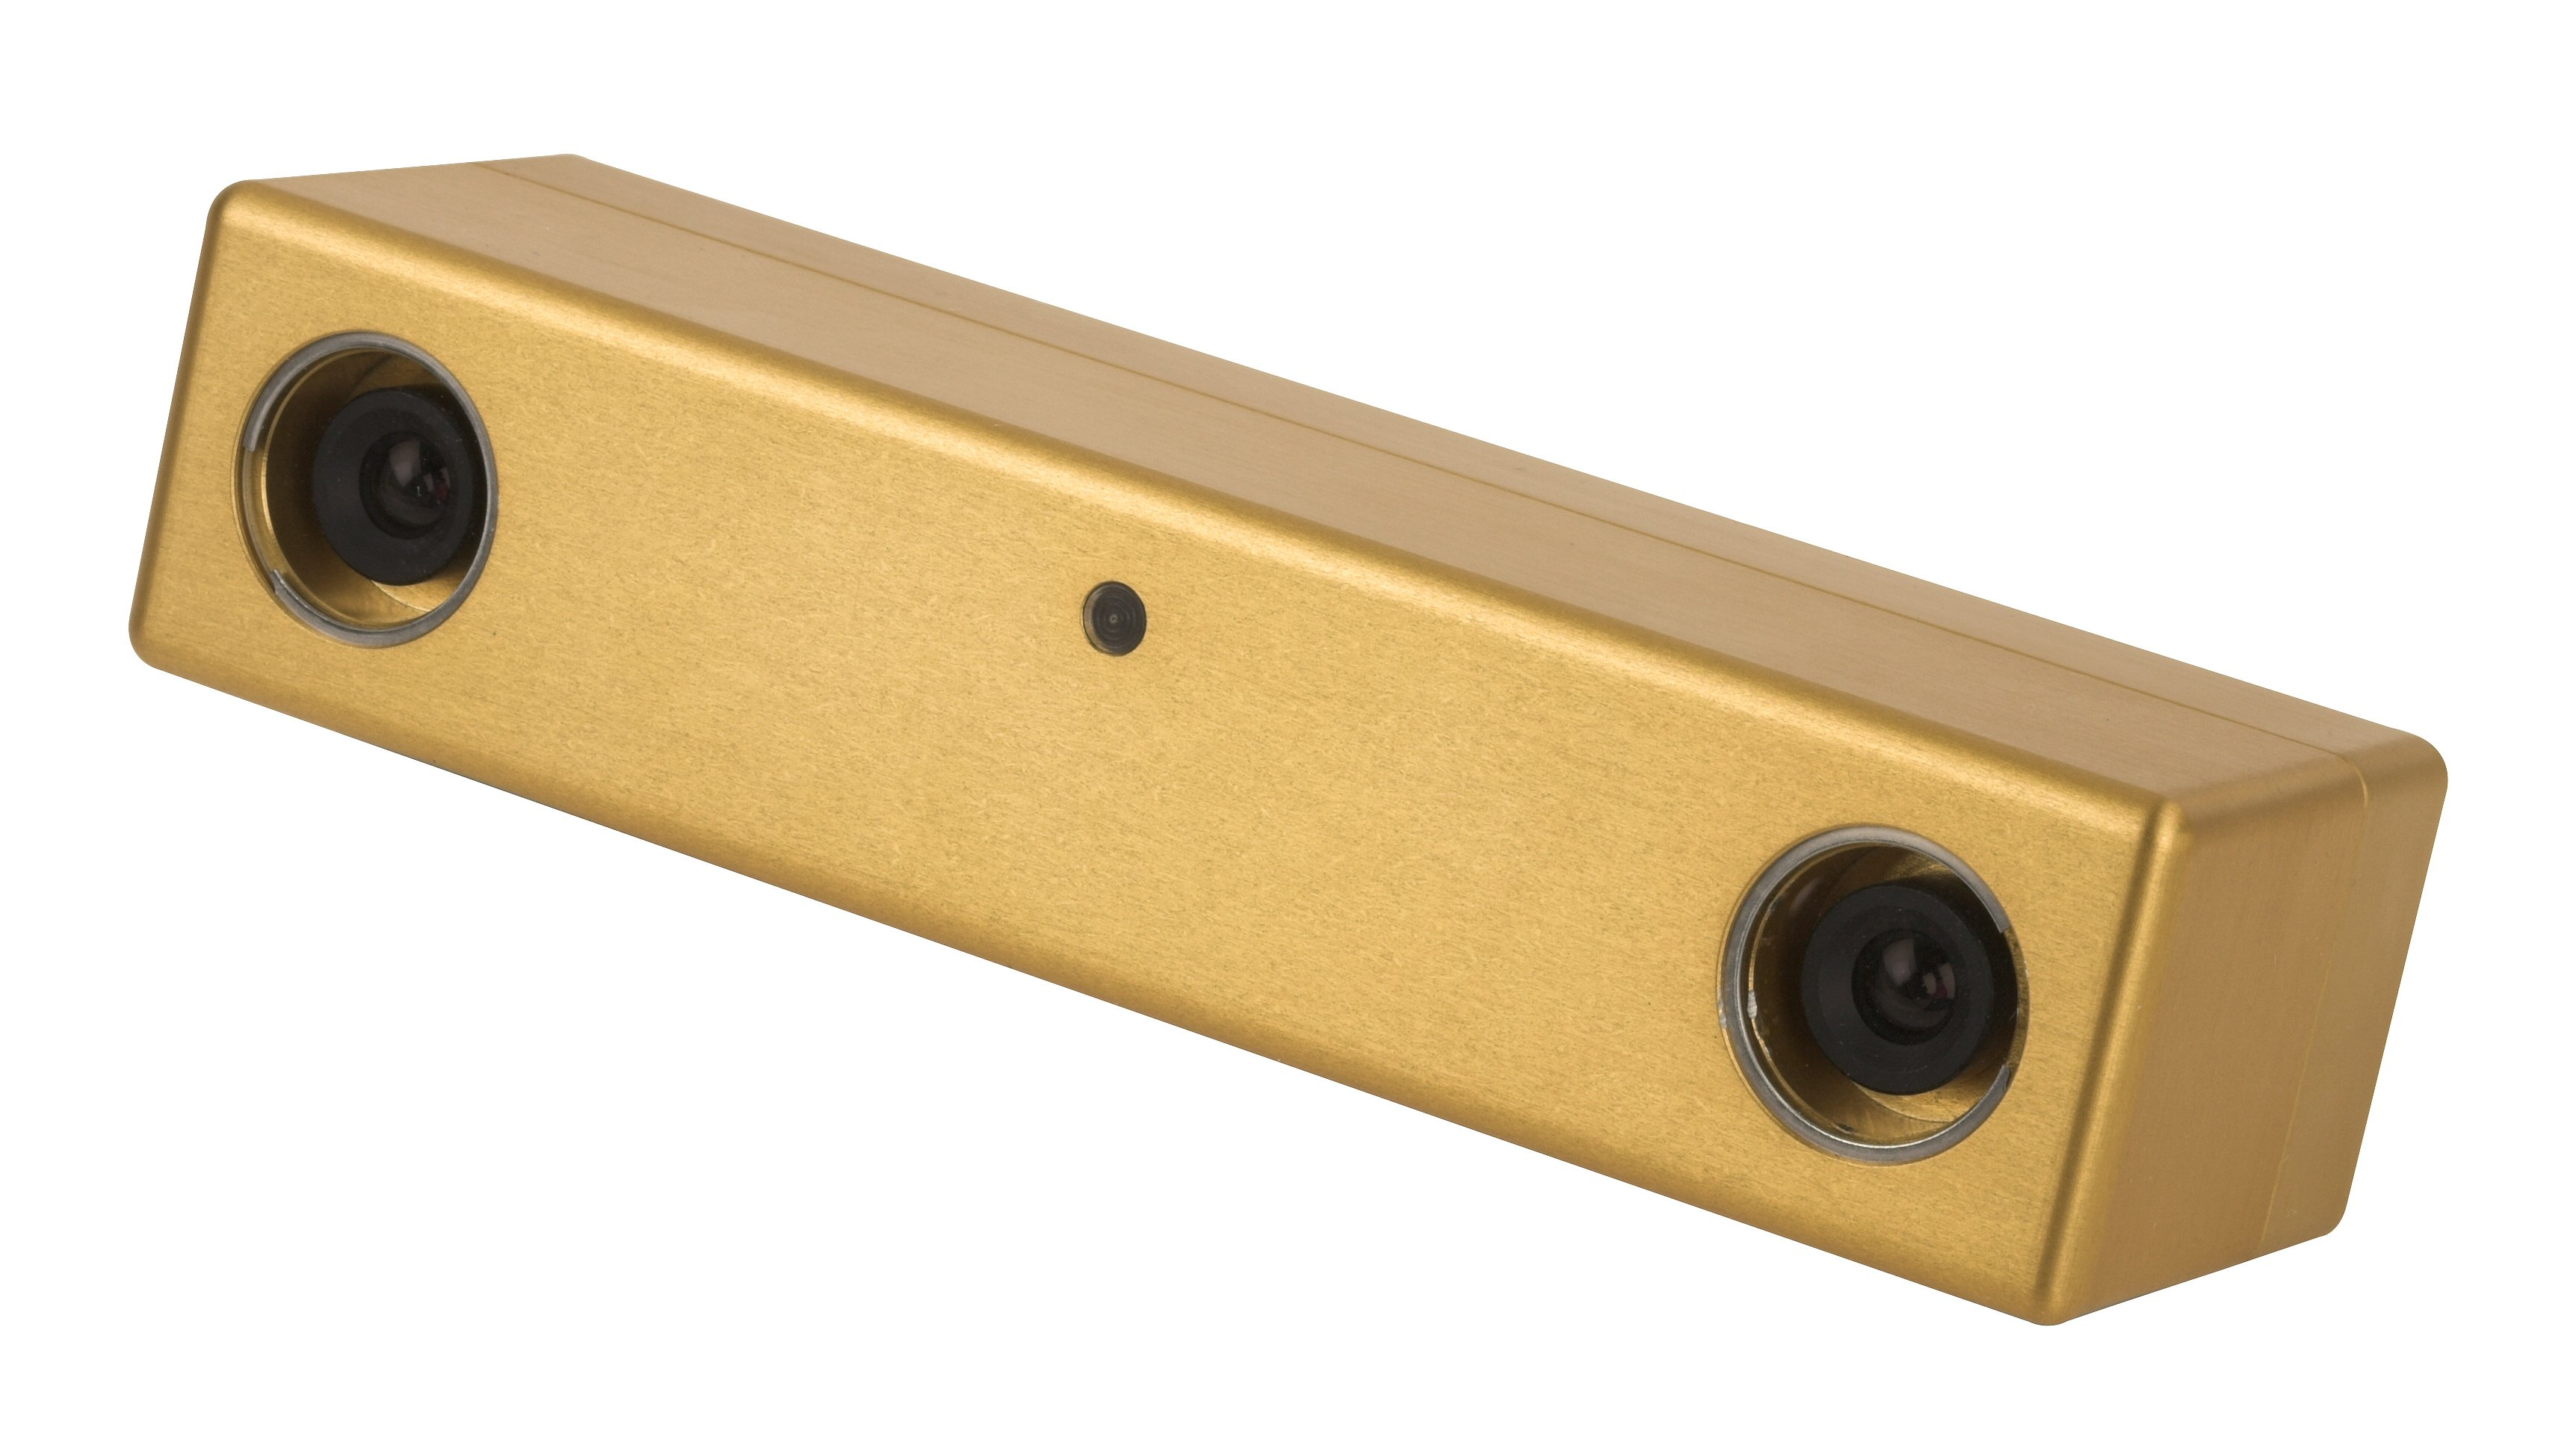
\includegraphics[width=0.5\linewidth]{images/bumblebee2.jpg}
  \caption[Exemple de caméra stereo]{Exemple de caméra stereo PointGrey Bumblebee2}
  \label{fig:stereo_camera}
\end{figure}

La vision stéréo est un sujet qui est étudié depuis longtemps pour diverses utilisations tel que la cueillette d'objets par bras manipulateur \citep{Hernandez2017}, l'effacement d'arrière-plan \citep{Kanade1996Stereo} et la navigation de robots \citep{Fraundorfer2012}. Sans aller dans les détails de la géométrie épipolaire permettant de trianguler un point dans l'espace, l'idée générale derrière la vision stereo est de comparer les images de deux caméras pour calculer la distance entre deux points correspondants. Cette distance, que l'on nomme la disparité, est directement liée à la position 3D du point dans le monde selon la relation
\begin{align}
  d = f \frac{B}{Z}
\end{align}
où $d$ est la disparité, $f$ est la longueur focale en pixels, $B$ est la distance entre les deux caméras et $Z$ est la profondeur du point. Diverses méthodes existent pour mettre en correspondance les points (ou plus souvent des blocs de plusieurs pixels) entre les deux images. Nous avons par exemple les algorithmes locaux cherchant le plus petit coût de correspondance suivant une métrique tel que la différence absolue ou la somme des différences au carré calculée sur l'intensité des pixels d'un bloc \citep{Szeliski2011}. Ces coûts locaux peuvent aussi être optimisés globalement par \textit{belief propagation} pour obtenir une image de disparité cohérente \citep{Klaus2006}. L'approche utilisée dans la librairie de traitement d'images OpenCV est en fait une approximation de l'optimisation globale où la programmation dynamique est utilisé pour optimiser une fonction d'énergie \citep{Hirschmuller2008}.

Cependant, peu importe l'algorithme utilisé, il sera toujours important d'avoir de la texture dans l'image, sans quoi il existera une incertitude sur la correspondance des blocs et le calcul de disparité échouera. Outre les filtres lisseurs tentant de remplir les trous dans une image de disparité où la recherche de correspondance aurait échoué, les avancées récentes dans le domaine tendent vers l'utilisation de l'apprentissage machine pour prédire l'image de disparité en entier \citep{Kendall_2017_ICCV}. \citep{meier2017real} proposent une solution plus classique où l'échec de correspondance est prédit et corrigé au moyen d'une caméra stereo secondaire placée orthogonalement à la caméra principale.

\subsection{Détection de lignes}

La méthode la plus connue pour la détection de contours dans une image reste à ce jour celle proposée par \citep{Canny1986} qui consiste brièvement en un calcul de gradient suivi d'une suppression des non-maxima. Avec la popularité grandissante de l'apprentissage machine, certaines nouvelles méthodes ont été proposées pour la détection de contours à base de réseaux de neurones. Par exemple, \textit{Holistically-Nested Edge Detection} proposé par \citep{Xie2015} est un réseau de neurones entièrement convolutionnel qui fait aussi usage d'apprentissage multi-échelle de caractéristiques imbriquées. L'avantage majeur des méthodes par apprentissage machine est qu'elles ne requièrent pas la calibration de paramètres.

Une fois les contours détectés et inscrits dans une image binarisée, il devient possible d'appliquer une transformée de Hough pour la détection de lignes droites \citep{Duda1972}. Avec le temps, plusieurs améliorations ont été proposées pour accélérer le calcul de la transformée, notamment l'introduction de méthodes probabilistes n'utilisant qu'un sous-ensemble des données pour la détection des lignes \citep{Matas2000}. \citep{Herout2013} dénombrait 39 variantes de la transformée de Hough incluant des variantes faisant usage de matériel spécialisé tel que des unités de traitement graphiques (GPU) ou des processeurs configurables (FPGA).

D'autres méthodes de détection de ligne ont aussi été proposées sans le besoin de passer par une transformée de Canny. Par exemple, le \textit{Line Segment Detector} de \citep{Gioi2012lsd} fonctionne par régions de support de ligne. D'un autre côté, EDLines proposé par \citep{AKINLAR20111633} fonctionne directement sur une image à tons de gris: des points d'ancrage sont calculés sur une image gradient pour effectuer un tracé de contours. LSD et EDLines ont tous les deux l'avantage d'être rapides et ont été conçus pour ne pas avoir besoin de réglage de paramètres.

% !TEX root = Document.tex
\section{Choix de capteurs}\label{sec:capteurs}
%\color{red}
%Intégrer ce chapitre à la revue de littérature? Ou faire un chapitre très court.
%\color{black}

Il va de soi que pour qu'un robot puisse éviter des obstacles et se déplacer de façon autonome, il doit avoir un moyen de percevoir son environnement. Dans ce chapitre, nous traitons des capteurs utilisables dans le contexte de la navigation de robots mobiles, et possiblement de la reconstruction 3D. En général, il existe trois capteurs couramment utilisés: la vision passive, la vision active et les télémètres laser.

\subsection{Systèmes de vision passive}

Dans la section \ref{subsec:stereo_vision}, nous avons touché au sujet de vision stéréo, qui est un exemple de premier plan d'un capteur passif, c'est-à-dire un capteur capable de percevoir un phénomène quelconque sans devoir émettre un signal. En effet, les caméras sont un moyen peu coûteux de percevoir la profondeur et sont couramment utilisées dans des micro-véhicules aériens commerciaux tel que le Yuneec Typhoon H de la Figure \ref{subfig:yuneec_full}. Par contre, la vision stéréo n'étant pas infaillible, la perception de profondeur peut échouer dans les environnement comportant peu de textures ou trop peu de lumière. Malgré certaines méthodes de régularisation pour tenter de remplir les trous en propageant l'information des régions aux alentours \citep{Hirschmuller2008}, l'état de l'art est à un point où les entreprises jugent encore prudent d'ajouter un capteur secondaire, tel qu'un sonar dans la (fig. \ref{subfig:yuneec_closeup}), pour compenser les échecs de perception.

\begin{figure}[ht]
  \centering
  \subfloat[]{
  	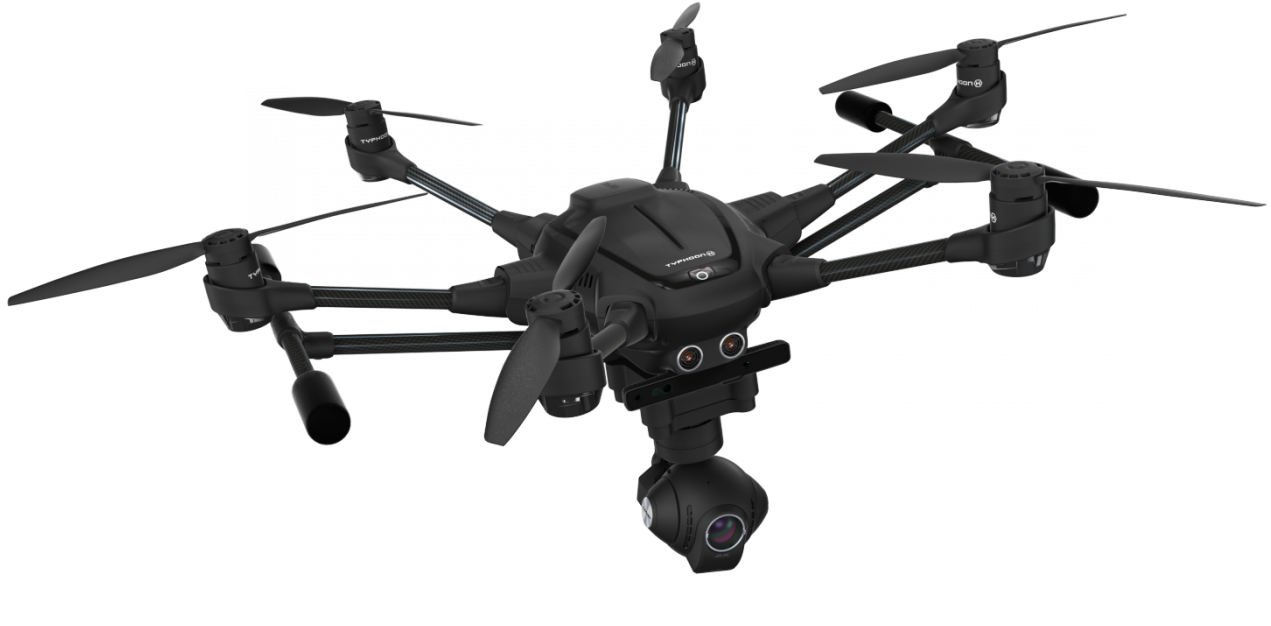
\includegraphics[width=0.60\linewidth]{images/yuneec_full.png}
  	\label{subfig:yuneec_full}
  }
  \hfil
  \subfloat[]{
  	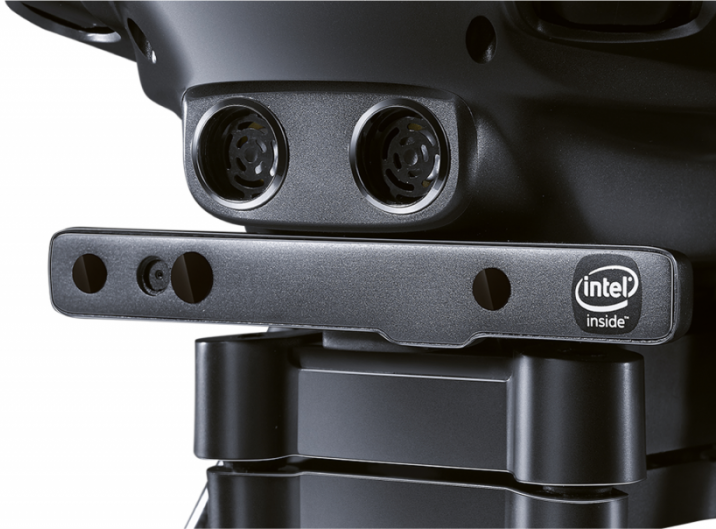
\includegraphics[width=0.35\linewidth]{images/yuneec_closeup.png}
  	\label{subfig:yuneec_closeup}
  }
  \caption[Systèmes de caméra stéréo augmentés de capteurs secondaires.]{
    (a) Le multi-rotor Yuneec Typhoon H (b) La caméra stéréo infrarouge Intel RealSense augmentée d'un sonar pour détecter les obstacles lors des échecs de perception.
  }
  \label{fig:yuneec}
\end{figure}

Dans le contexte des micro-véhicules aériens, il arrive parfois que l'on veuille miniaturiser et simplifier le système à un point où il serait désirable d'avoir un système monoculaire au lieu d'un système stéréo. Tel que mentionné dans la section \ref{subsec:reconstruction}, il est possible de mettre à l'échelle une carte 3D construite monoculairement au moyen d'une source d'information métrique secondaire tel qu'une centrale inertielle \citep{muratal2017vimonoslam}. Par contre, pour que cette carte soit utilisable pour la navigation, elle doit être construite de façon à pouvoir représenter les surfaces des obstacles. \citep{Yang2017} proposent de profiter de l'exactitude d'un système d'odométrie visuo-inertiel pour construire des cartes de profondeur au moyen de résolution stéréo par mouvement. En d'autres mots, au lieu d'avoir deux caméras pour la triangulation de points, nous avons une seule caméra qui se déplace dans l'espace pour la triangulation.

\subsection{Systèmes de vision active}

Une autre façon de compenser pour les lacunes de la vision stéréo est d'utiliser la vision active, c'est-à-dire de projeter une onde quelconque pour en détecter le retour. L'un des exemples les mieux connus de ce type de système est la ligne de produits Microsoft Kinect. Originalement prévue pour permettre aux usager des consoles de jeux Xbox360 de jouer à des jeux contrôlés par gestuelle, la caméra de profondeur a rapidement été adoptée par le milieu académique pour son faible coût et sa précision relativement élevée \citep{khoshelham2012}. La Kinect pour Xbox360 fonctionnait originalement au moyen d'un projecteur laser quasi-infrarouge (NIR) et d'une caméra NIR. Suivant le principe de la \guillemotleft lumière structurée \guillemotright un motif NIR connu est projeté sur la scène et une caméra analysant la déformation du motif permet de calculer la profondeur de la scène \citep{Zhang2012}.

\begin{figure}[!h]
  \centering
  \subfloat[]{
    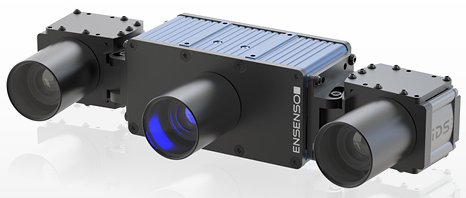
\includegraphics[width=0.5\linewidth]{images/ensenso3d.jpg}
    \label{subfig:ensenso}
  }
  \subfloat[]{
    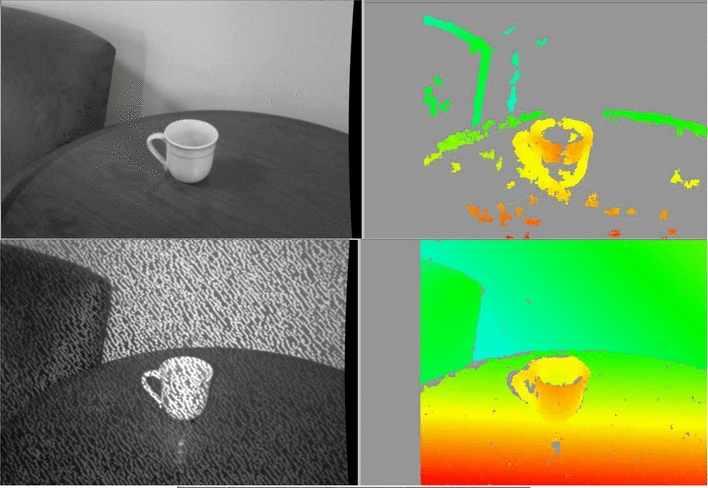
\includegraphics[width=0.4\linewidth]{images/konolidge_stereo.jpg}
    \label{subfig:kono_stereo}
  }
  \caption[Caméras 3D par projection de texture]{
    (a) Caméra Ensenso 3D fonctionnant par projection de texture et résolution stéréo.
    (b) Résultat de la méthode proposée par \citep{konolige2010}.
  }
  \label{fig:3d_cams}
\end{figure}

\citep{konolige2010} propose une méthode similaire où une caméra stéréo est augmentée d'un projecteur de texture pour permettre la résolution de la profondeur dans les scènes dépourvues de texture adéquate. La mise en correspondance des blocs stéréo se fait avec la connaissance \textit{a priori} de la texture qui avait été projetée. À ce jour, ce principe est utilisé dans une variété de produits commerciaux tel que la caméra Ensenso 3D de IDS Imaging.

Par contre, les caméras par lumière structurée souffrent de plusieurs inconvénients, notamment leur sensibilité à la lumière infrarouge ambiante et leur imprécision dans le cas de scènes en mouvement \citep{khoshelham2012}. Durant les cinq dernières années, nous avons assisté à une baisse de prix considérable dans les capteurs de profondeur fonctionnant par \textit{time-of-flight (ToF)} (temps de vol). Le principe du ToF se résume à projeter périodiquement une lumière NIR modulée en intensité et d'en mesurer le temps de retour. Bien sûr, cette dernière n'est pas mesurée directement; elle est plutôt calculée à partir du déphasage du signal de retour capté par la caméra. L'avantage de caméras ToF est qu'elles offrent une bonne performance dans des environnements à haute et basse luminosité, en plus d'offrir un temps de réponse rapide. Encore ici, l'exemple le plus répandu d'une caméra ToF est la Microsoft Kinect v2 pour Xbox One.

Une dernière amélioration récente dans le domaine des caméras de profondeur est la ligne de produits Intel RealSense (ex. Fig. \ref{subfig:yuneec_closeup}) fonctionnant par lumière non-structurée (\emph{unstructured light}) dont le traitement est accéléré par un circuit intégré à application dédiée (ASIC). Une texture fixe est projetée sur la scène au moyen d'un projecteur laser infrarouge. Cette texture est précalculée pour maximiser le contraste et pour minimiser la similitude le long de l'axe de recherche épipolaire. À l'inverse de la Kinect 1, la texture est inconnue au moment de la résolution stéréo et ne sert que d'aide secondaire au système. L'originalité de la solution provient du fait que la caméra stéréo infrarouge permet d'opérer une RealSense dans un environnement où la lumière du soleil est de forte intensité ainsi que dans la noirceur totale grâce au projecteur. De plus, la nature matérielle des caméras stéréo fait en sorte que la RealSense peut être produite à faible coût, dans un petit emballage et avec une consommation électrique relativement basse \citep{Keselman_2017_CVPR_Workshops}.

\subsection{Télémètres laser}

Un dernier type de capteur à considérer est le télémètre laser ou LIDAR pour \textit{Light Detection and Ranging}. Opérant souvent par ToF, les télémètres lasers sont combinés à des assemblages de moteurs et de miroirs pour obtenir des scanners laser en 2D ou 3D. L'un des exemples les plus médiatisés de l'utilisation de lidars pour la navigation de véhicules terrestres était Stanley, la voiture autonome de Stanford qui a gagné le DARPA Grand Challenge en 2005 \citep{thrun2006stanley}.

\begin{figure}[ht]
  \centering
  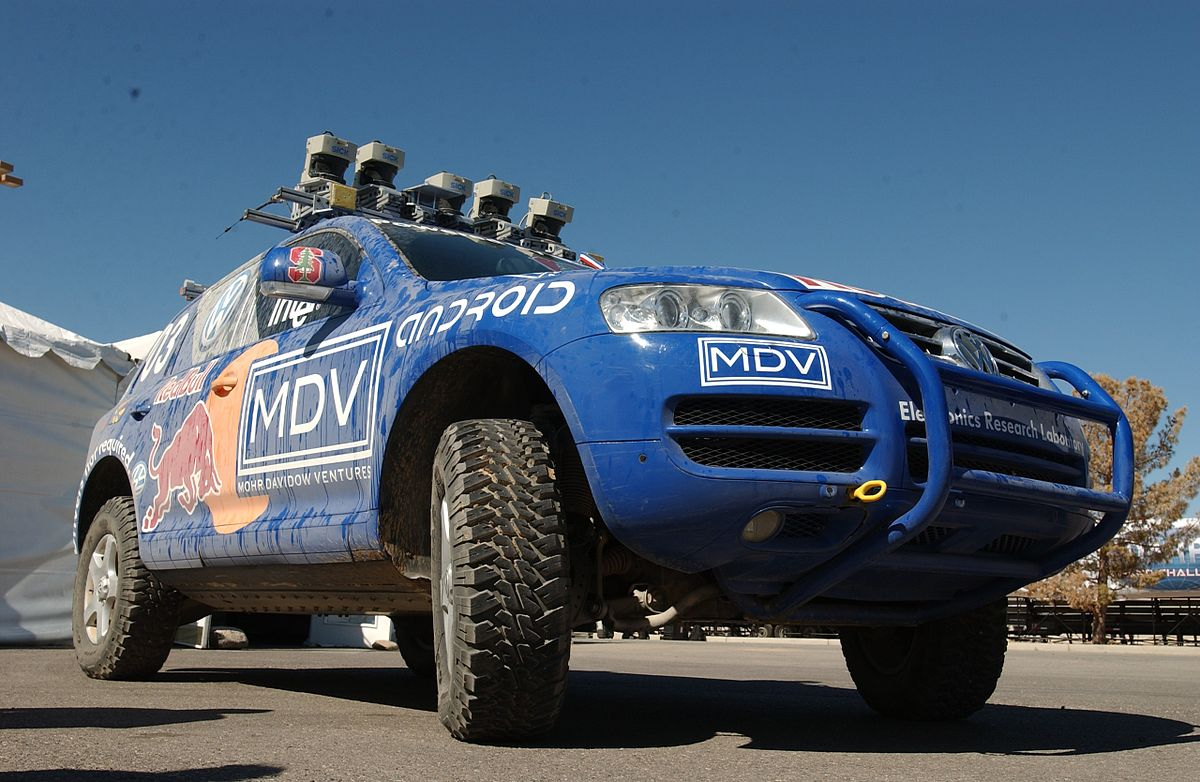
\includegraphics[width=0.5\linewidth]{images/stanley.jpg}
  \caption[Stanley la voiture autonome fonctionnant par lidar.]{Stanley était équipé de 5 lidar 2D sur son toit pour la détection d'obstacles et la navigation \citep{thrun2006stanley}.}
  \label{fig:stanley}
\end{figure}

Avec le temps, les lidars se sont améliorés pour devenir plus compacts et moins dispendieux à un point où il est possible de les installer sur des véhicules multi-rotors pour fins de cartographie et de localisation \citep{zhang2018aerial}. La tendance de miniaturisation se maintient avec l'arrivée récente sur le marché de lidars à état solide sans moteurs ou miroirs pour la déflection du faisceau laser. Dans le chapitre \ref{sec:uav} nous démontrerons l'utilisation d'un tel capteur, le LeddarVu8 pour la navigation d'un véhicule aérien.

\begin{figure}[!h]
  \centering
  \subfloat[]{
    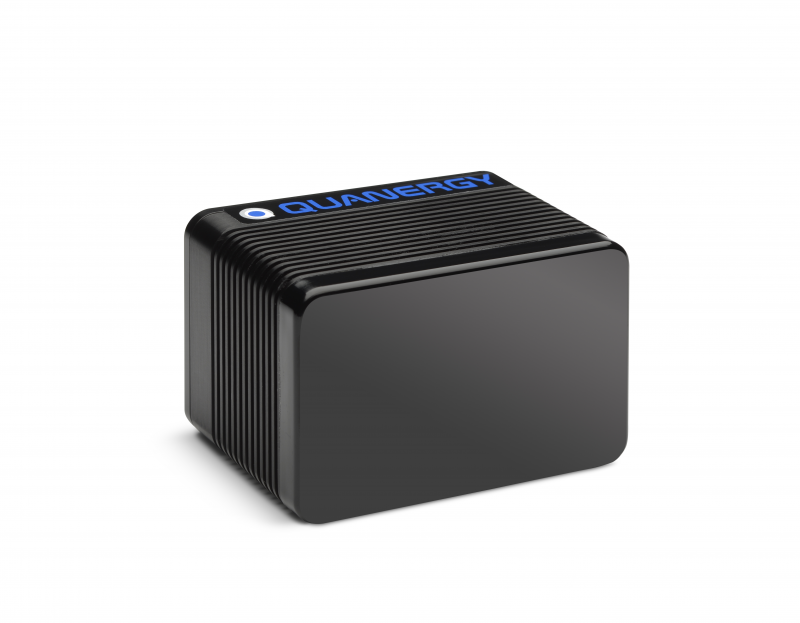
\includegraphics[width=0.5\linewidth]{images/quanergy.png}
    \label{subfig:quanergy}
  }
  \subfloat[]{
    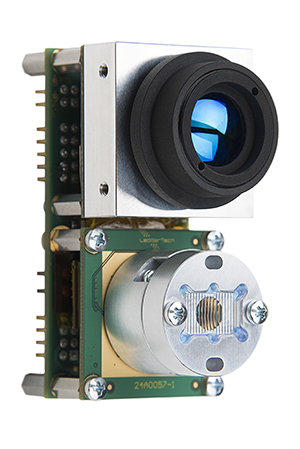
\includegraphics[width=0.2\linewidth]{images/leddar.jpg}
    \label{subfig:leddarvu}
  }
  \caption[Lidars à état solide]{
    (a) Le Quanergy S3 avec $8000$ points dans un angle de vue de $120^\circ$ horizontal et vertical \citep{eldada2016}.
    (b) Le LeddarVu8 avec $8$ segments de détection.
  }
  \label{fig:lidars}
\end{figure}
